% FISAT 2026, paper 367005: supplementary material (29 Oct 2026). Build main.tex first; section, table and
% equation numbers of the paper are read from main.aux.
\documentclass[runningheads]{llncs}
\usepackage[T1]{fontenc}
\usepackage{graphicx}
\usepackage{array}
\usepackage{flafter} % a float never appears before the text that defines it
\usepackage{float} % [H] keeps the appendix tables and figures in reading order
\usepackage{amsmath}
\usepackage{listings}
\usepackage{tikz}
\usetikzlibrary{arrows.meta}
\usepackage{xr-hyper}
\externaldocument[P-]{main}
\usepackage{hyperref}
\usepackage{url}
\usepackage{microtype}
\urlstyle{same}
\Urlmuskip=0mu plus 1mu % lets long URLs break after "/" instead of running into the margin
\hypersetup{hidelinks} % no coloured boxes around citations and links
\setlength{\tabcolsep}{6pt} % llncs sets 1.4pt, which runs table columns together
\setlength{\emergencystretch}{1em} % allows a looser line rather than one that runs into the margin

\lstset{basicstyle=\ttfamily\footnotesize,breaklines=true,frame=none,columns=fullflexible,keepspaces=true,numberbychapter=false}

\renewcommand{\thesection}{S\arabic{section}}
\renewcommand{\thetable}{S\arabic{table}}
\renewcommand{\thefigure}{S\arabic{figure}}
\AtBeginDocument{\renewcommand{\thelstlisting}{S\arabic{lstlisting}}}

\begin{document}

\title{Supplementary Material for ``Evaluating GPT-5.4-mini for Gherkin Test Generation: An Empirical Study''}
\titlerunning{Evaluating GPT-5.4-mini for Gherkin Test Generation: Supplement}

\author{Nguyen Minh Hoang \and Nguyen Hieu An \and Le Thi Quynh Chi\thanks{Corresponding author.}}
\authorrunning{N. M. Hoang et al.}
\institute{FPT University, Vietnam\\ \email{chiltq6@fe.edu.vn}}

\maketitle

\noindent This supplement belongs to the paper above. Section, table, figure and reference numbers without the prefix S refer to the paper; the references are those of the paper.

\appendix

\section{Prompt, Skeleton Example and Additional Results}
\label{app:details}

Listing~\ref{lst:prompt} gives the prompt template of condition C0 (Section~\ref{sec:method}), Table~\ref{tab:skeleton} illustrates the skeleton extraction of Section~\ref{sec:metric1}, Fig.~\ref{fig:dist} and Fig.~\ref{fig:domain} show the distribution of skeleton cosine in C0 overall and per project, Table~\ref{tab:sweep} gives the threshold sensitivity analysis of Section~\ref{sec:res-b3}, and Table~\ref{tab:rq2} gives the parser results of RQ2.

\begin{lstlisting}[caption={Prompt template of condition C0. Braced placeholders are instantiated by project at run time.},label={lst:prompt}]
System: {domain_specific_system_message}
User:
Generate a BDD Gherkin file for the following user story.
Follow the exact style, wording, and conventions shown in the Example.

EXAMPLE USER STORY:
{example_user_story_from_same_domain}

EXAMPLE GHERKIN:
{example_gherkin_from_same_domain}

---
NOW GENERATE FOR THIS USER STORY:
{user_story_text}
\end{lstlisting}

\begin{table}[t]
\centering
\caption{Skeleton extraction on a short Sylius-style fragment.}
\label{tab:skeleton}
\scriptsize
\begin{tabular}{ll}
\hline
Original line & Skeleton line\\
\hline
\texttt{@ui} & (removed)\\
\texttt{Given a product "T-Shirt" priced at "\$20.00"} & \texttt{Given a product <PARAM> priced at <PARAM>}\\
\texttt{When I add 3 units to the cart} & \texttt{When I add <NUM> units to the cart}\\
\texttt{| name | price |} & (removed)\\
\texttt{Then the total should be "\$60.00"} & \texttt{Then the total should be <PARAM>}\\
\hline
\end{tabular}
\end{table}

\begin{figure}[t]
\centering
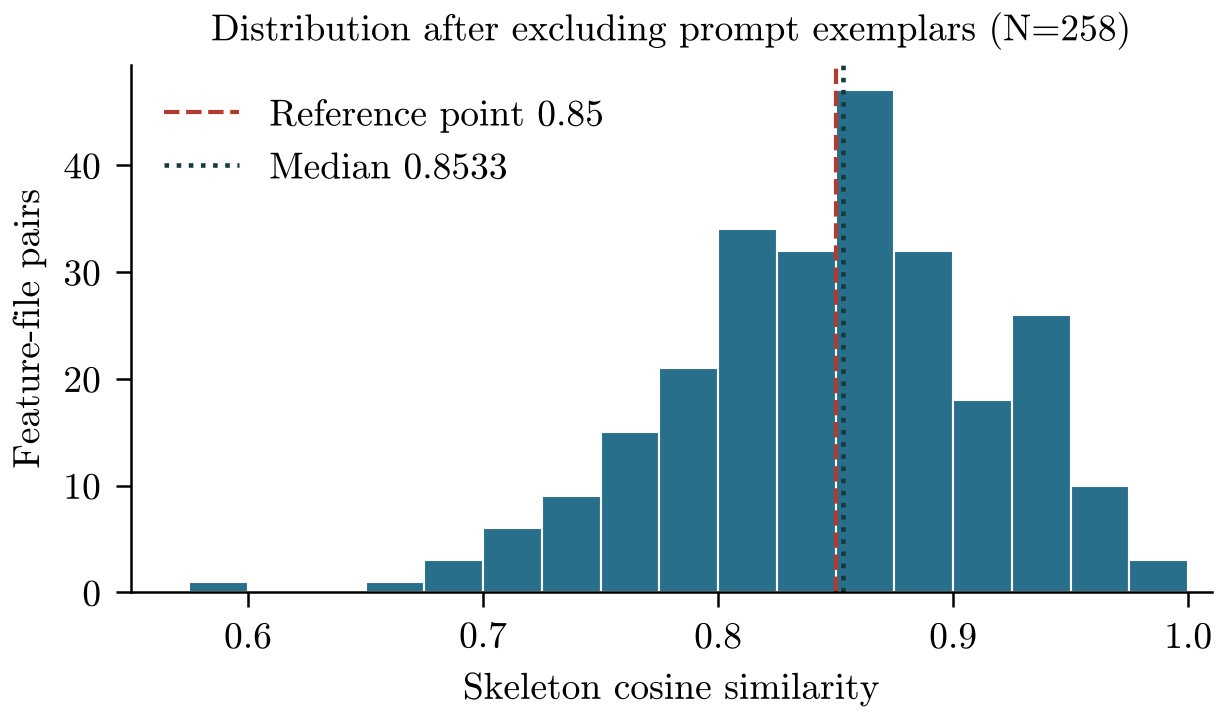
\includegraphics[width=0.72\textwidth]{figures/fig1_skeleton_distribution_258.png}
\caption{Distribution of skeleton cosine similarity for the 258 non-exemplar files (condition C0).}
\label{fig:dist}
\end{figure}

\begin{figure}[t]
\centering
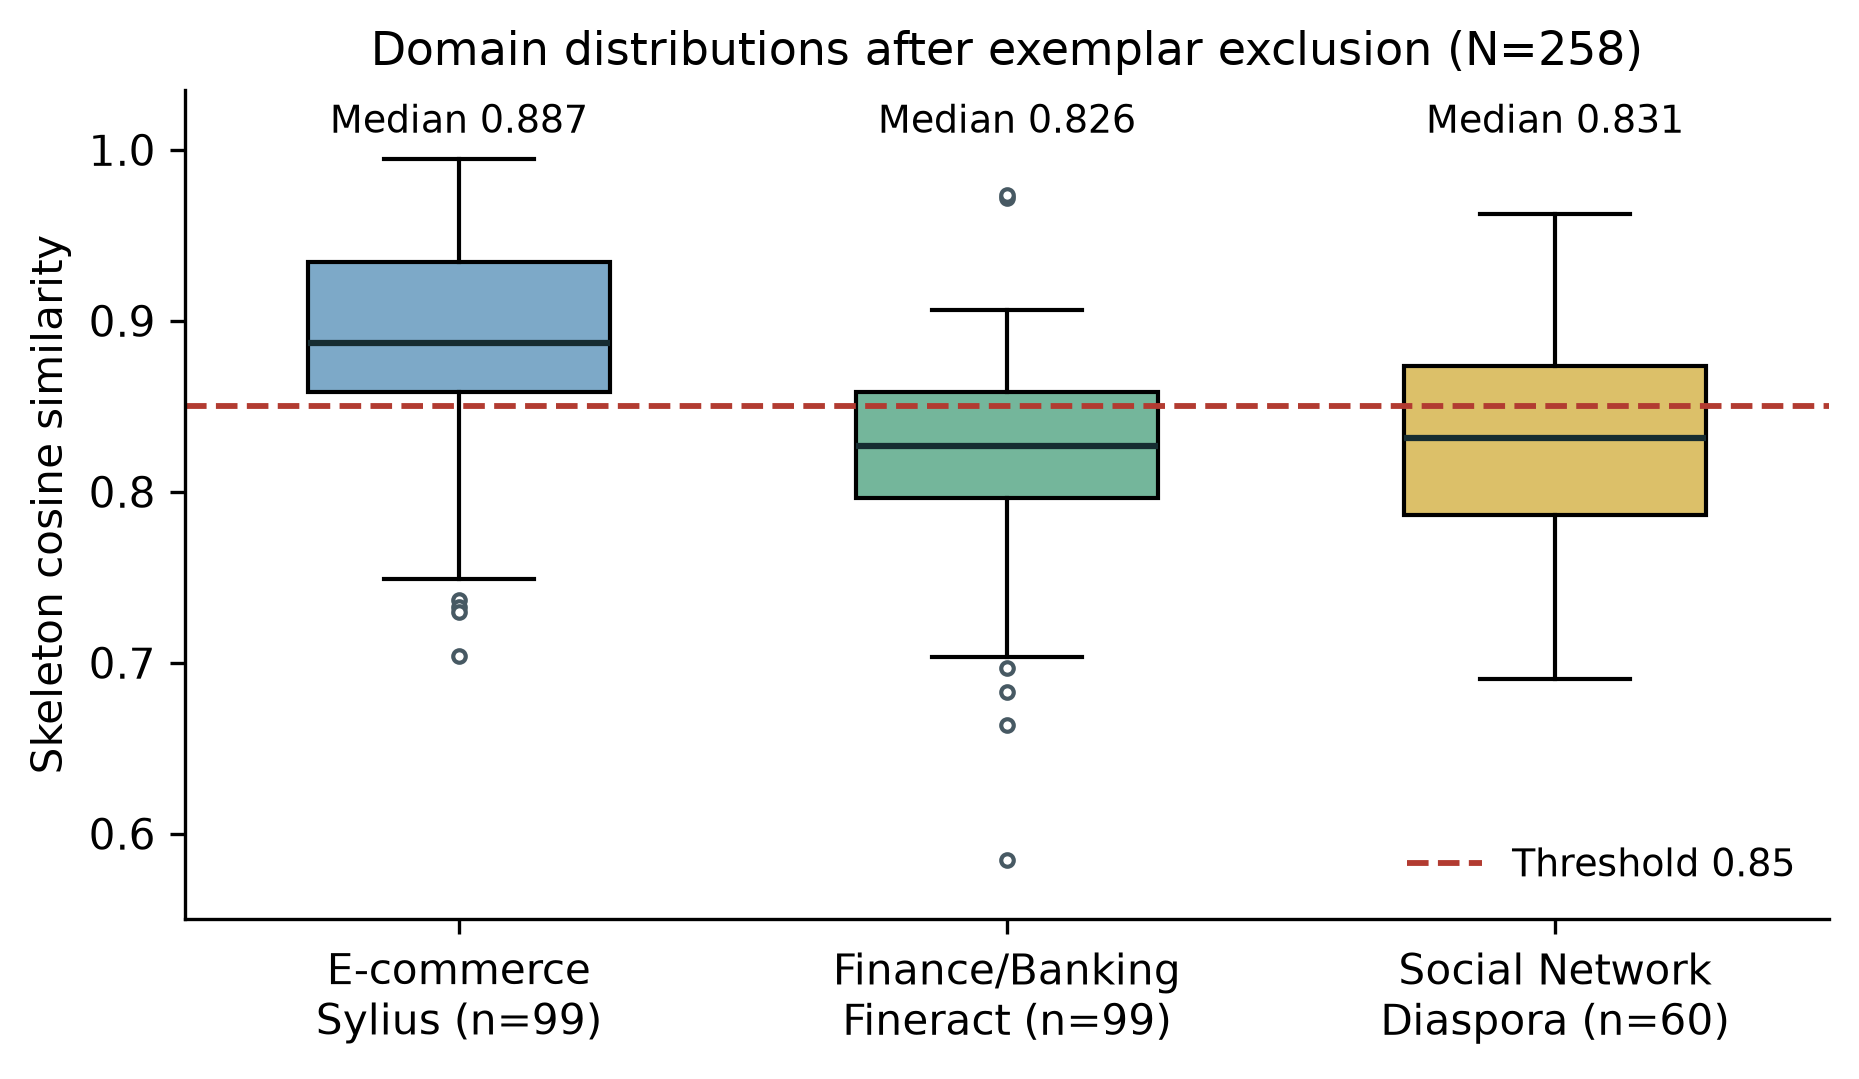
\includegraphics[width=0.72\textwidth]{figures/fig2_domain_distributions_258.png}
\caption{Skeleton cosine similarity per project (C0, $N = 258$). The dashed line marks 0.85.}
\label{fig:domain}
\end{figure}

\begin{table}[t]
\centering
\caption{Threshold sensitivity (C0, $N = 258$). The $p$-value is the one-sided Wilcoxon test that the median exceeds $t$.}
\label{tab:sweep}
\begin{tabular}{rrrrrrr}
\hline
$t$ & Share $\ge t$ [95\% CI] & Median $- t$ & $p$ & Sylius & Fineract & Diaspora\\
\hline
0.80 & 78.3\% [72.8, 83.2] & $+0.053$ & $< 0.001$ & 91.9\% & 73.7\% & 63.3\%\\
0.82 & 67.8\% [61.8, 73.5] & $+0.033$ & $< 0.001$ & 87.9\% & 56.6\% & 53.3\%\\
0.84 & 59.3\% [53.0, 65.4] & $+0.013$ & 0.010 & 84.8\% & 40.4\% & 48.3\%\\
0.85 & 52.7\% [46.4, 58.9] & $+0.003$ & 0.474 & 77.8\% & 34.3\% & 41.7\%\\
0.86 & 43.4\% [37.3, 49.7] & $-0.007$ & 0.988 & 73.7\% & 22.2\% & 28.3\%\\
0.88 & 30.6\% [25.1, 36.6] & $-0.027$ & 1.000 & 55.6\% & 12.1\% & 20.0\%\\
0.90 & 22.1\% [17.2, 27.7] & $-0.047$ & 1.000 & 45.5\% & 4.0\% & 13.3\%\\
\hline
\end{tabular}
\end{table}

\begin{table}[t]
\centering
\caption{Parser compliance of condition C0 (behave 1.3.3 parser).}
\label{tab:rq2}
\begin{tabular}{lrr}
\hline
Statistic & $N = 258$ (primary) & $N = 261$\\
\hline
Parser PASS / FAIL & 255 / 3 & 258 / 3\\
ESR & 98.84\% & 98.85\%\\
95\% Clopper--Pearson CI & [96.64\%, 99.76\%] & [96.68\%, 99.76\%]\\
Exact binomial $p$ ($p_0 = 0.80$) & $4.6 \times 10^{-21}$ & $2.4 \times 10^{-21}$\\
\hline
\end{tabular}
\end{table}

\clearpage
\section{Perturbation Test}
\label{app:perturb}

\textbf{Design.} The perturbation test measured whether the metric reacts to seeded defects. From the reference files, 120 scenarios (40 per project, fixed seed) were extracted, and eight operators were applied where applicable: changing a number, a quoted value, a comparison operator or a negation, dropping a Then or a Given step, swapping a When with a Then, and moving a Then to the front. Each mutant was compared with its original scenario using the same skeleton metric.

\textbf{Results.} The 120 extracted scenarios yielded 683 applicable mutants. Of these, 29 mutants do not parse, and the extraction omitted the Background of 74 of the 120 source scenarios. Restricting to the 623 pairs in which both texts parse and the original has no keyword-order flag, every mutant keeps a skeleton cosine of at least 0.8995 with its original. At 0.90, 622 of 623 mutants would still pass, and at 0.95, 97.9\%. For changed numbers and quoted values (179 pairs) the skeletons are identical, which follows from masking and is not an empirical finding. Swapped When/Then steps and Then steps moved to the front (210 pairs) score at least 0.954, although the keyword-order check flags all of them. Because the test compares single scenarios and the main metric compares whole files, these results show insensitivity at the scenario level and do not estimate a false-negative rate for whole files.


% Reference list transcribed verbatim from the camera-ready PDF (10 Aug 2026).
% The PDF list is in citation order with title-case titles and full initials,
% which splncs04.bst does not produce, so the list is kept as thebibliography.
% Revision: DOI added to clopper1934; cohen1960, kruskal1952, holm1979 added. Titles, volumes,
% issues, pages and DOIs of these four were checked against Crossref (18 Oct 2026); holm1979 has
% no DOI and was checked against the GESIS record and its JSTOR stable URL.
\begin{thebibliography}{99}

\bibitem{rathnayake2026}
Rathnayake, A., Shahin, M., Abaei, G.: Behaviour Driven Development Scenario Generation with Large Language Models. arXiv:2603.04729 (2026). \url{https://doi.org/10.48550/arXiv.2603.04729}

\bibitem{karpurapu2024}
Karpurapu, S., Myneni, S., Nettur, U., Gajja, L.S., Burke, D., Stiehm, T., Payne, J.: Comprehensive Evaluation and Insights Into the Use of Large Language Models in the Automation of Behavior-Driven Development Acceptance Test Formulation. IEEE Access 12 (2024). \url{https://doi.org/10.1109/ACCESS.2024.3391815}

\bibitem{ferreira2025}
Ferreira, M., Viegas, L., Faria, J.P., Lima, B.: Acceptance Test Generation with Large Language Models: An Industrial Case Study. In: IEEE/ACM International Workshop on Automation of Software Test (AST) (2025). arXiv:2504.07244

\bibitem{fernandes2025}
Fernandes, H., Perkusich, M., Albuquerque, D., Silva, I., Santos, D.F.S., Gorgonio, K., Perkusich, A.: A Comparative Study of LLMs for Gherkin Generation. In: Brazilian Symposium on Software Engineering (SBES), pp. 171--181 (2025). \url{https://doi.org/10.5753/SBES.2025.9888}

\bibitem{fonseca2025}
Fonseca, P.L., Lima, B., Faria, J.P.: Streamlining Acceptance Test Generation for Mobile Applications Through Large Language Models: An Industrial Case Study. In: 40th IEEE/ACM International Conference on Automated Software Engineering (ASE) (2025). \url{https://doi.org/10.1109/ASE63991.2025.00273}

\bibitem{zhang2025testbench}
Zhang, Q., Shang, Y., Fang, C., Gu, S., Yu, S., Zhou, J., Chen, Z.: TestBench: Evaluating Class-Level Test Case Generation Capability of Large Language Models. Frontiers of Computer Science 21(6), 2106202 (2027), published online 13 October 2025. \url{https://doi.org/10.1007/s11704-025-50078-9}

\bibitem{chang2025}
Chang, H.-F., Shokrolah Shirazi, M.: A Systematic Approach for Assessing Large Language Models' Test Case Generation Capability. Software 4(1), 5 (2025). \url{https://doi.org/10.3390/software4010005}

\bibitem{wang2024xuat}
Wang, Z., Wang, W., Li, Z., Wang, L., Yi, C., Xu, X., Cao, L., Su, H., Chen, S., Zhou, J.: XUAT-Copilot: Multi-Agent Collaborative System for Automated User Acceptance Testing with Large Language Model. arXiv:2401.02705 (2024). \url{https://doi.org/10.48550/arXiv.2401.02705}

\bibitem{reimers2019}
Reimers, N., Gurevych, I.: Sentence-BERT: Sentence Embeddings using Siamese BERT-Networks. In: EMNLP-IJCNLP, pp. 3982--3992 (2019). \url{https://doi.org/10.18653/v1/D19-1410}

\bibitem{cohen1960}
Cohen, J.: A Coefficient of Agreement for Nominal Scales. Educational and Psychological Measurement 20(1), 37--46 (1960). \url{https://doi.org/10.1177/001316446002000104}

\bibitem{arcuri2011}
Arcuri, A., Briand, L.C.: A Practical Guide for Using Statistical Tests to Assess Randomized Algorithms in Software Engineering. In: 33rd International Conference on Software Engineering, pp. 1--10 (2011). \url{https://doi.org/10.1145/1985793.1985795}

\bibitem{agresti2002}
Agresti, A.: Categorical Data Analysis, 2nd edn. John Wiley \& Sons (2002). \url{https://doi.org/10.1002/0471249688}

\bibitem{clopper1934}
Clopper, C.J., Pearson, E.S.: The Use of Confidence or Fiducial Limits Illustrated in the Case of the Binomial. Biometrika 26(4), 404--413 (1934). \url{https://doi.org/10.1093/biomet/26.4.404}

\bibitem{kruskal1952}
Kruskal, W.H., Wallis, W.A.: Use of Ranks in One-Criterion Variance Analysis. Journal of the American Statistical Association 47(260), 583--621 (1952). \url{https://doi.org/10.1080/01621459.1952.10483441}

\bibitem{holm1979}
Holm, S.: A Simple Sequentially Rejective Multiple Test Procedure. Scandinavian Journal of Statistics 6(2), 65--70 (1979). \url{https://www.jstor.org/stable/4615733}

\end{thebibliography}


\end{document}
